\documentclass[a4paper,12pt,oneside,openany,table,xcdraw]{article}

\usepackage{setspace}
\usepackage{multirow}
\usepackage{hyperref}
\usepackage{caption}
\usepackage{indentfirst}
\usepackage{tikz} %% fasores
\usetikzlibrary{arrows,arrows.meta,quotes,angles}
\usepackage{siunitx}

\usepackage[brazilian]{babel}
\usepackage[utf8x]{inputenc}
\usepackage{amsmath, graphicx, subfig, enumerate}
\usepackage{float, verbatim}
\usepackage[colorinlistoftodos]{todonotes}
\usepackage{makeidx}
\usepackage{geometry}

\graphicspath{{img/}}
\geometry{a4paper, hmargin={3cm, 3cm}, vmargin={3cm, 2cm} }
\setlength{\parindent}{1.0cm}
\captionsetup{font=small}

\usepackage{mathtools,listings} %%
\usepackage{color} %red, green, blue, yellow, cyan, magenta, black, white
\definecolor{mygreen}{RGB}{28,172,0} % color values Red, Green, Blue
\definecolor{mylilas}{RGB}{170,55,241}
\usepackage{listingsutf8}

\begin{document}
\newcommand{\thedepartment}{Faculdade de Engenharia Elétrica}
\newcommand{\thecourse}{FEELT}
\newcommand{\thetitle}{Resolução da Lista de Exercícios Extras}
\newcommand{\thetype}{Trabalho de Sinais e Sistemas II}
\newcommand{\theproftitle}{Bacharel em Engenharia Elétrica}
\newcommand{\thestudent}{Lesly Viviane Montúfar Berrios\\
\centering11811ETE001}
\newcommand{\theadvisor}{Prof. Alan Petrônio Pinheiro}
\newcommand{\thecity}{Uberlândia}

\thispagestyle{empty}\newcommand*{\themonth}{\ifthenelse{\the\month < 2}{Janeiro }
                  {\ifthenelse{\the\month < 3}{Fevereiro }
                  {\ifthenelse{\the\month < 4}{Março }
                  {\ifthenelse{\the\month < 5}{Abril }
                  {\ifthenelse{\the\month < 6}{Maio }
                  {\ifthenelse{\the\month < 7}{Junho }
                  {\ifthenelse{\the\month < 8}{Julho }
                  {\ifthenelse{\the\month < 9}{Agosto }
                  {\ifthenelse{\the\month < 10}{Setembro }
                  {\ifthenelse{\the\month < 11}{Outubro }
                  {\ifthenelse{\the\month < 12}{Novembro }{Dezembro }}}}}}}}}}}}
                  
\begin{titlepage}
\begin{center}

	\vspace{-0.5cm}

  \begin{figure}[hbt!]
		\begin{center}
		   
\includegraphics[width=2.8cm]{ufu-logo.png}
		\end{center}
	\end{figure}
 	%\vspace{-4cm}

%\begin{doublespacing}

  \Large{\textbf{Universidade Federal de Uberlândia}}\\
  \large{\thedepartment}\\
  \large{\thecourse}\\


\vspace{5.8cm}
  \par
  \large\textbf{\thetitle}
\vspace{5.8cm} 

%\end{doublespacing}
  \par
  \thetype\\
  por\\
  %\hspace{2cm}\large{}\\

\vspace{0.8cm}
\par
  \normalsize{\thestudent}\\ [2cm]
  \theadvisor

\par\vfill
  \thecity, \themonth / \the\year

\end{center}

\end{titlepage}

\lstset{language=Matlab,%
	inputencoding=utf8/latin1,
    %basicstyle=\color{red},
    breaklines=true,%
    morekeywords={matlab2tikz},
    keywordstyle=\color{blue},%
    morekeywords=[2]{1}, keywordstyle=[2]{\color{black}},
    identifierstyle=\color{black},%
    stringstyle=\color{mylilas},
    commentstyle=\color{mygreen},%
    showstringspaces=false,%without this there will be a symbol in the places where there is a space
    numbers=left,%
    numberstyle={\tiny \color{black}},% size of the numbers
    numbersep=9pt, % this defines how far the numbers are from the text
    emph=[1]{for,end,break},emphstyle=[1]\color{red}, %some words to emphasise
    %emph=[2]{word1,word2}, emphstyle=[2]{style},    
}

%% Comeca o documento !

\onehalfspacing
\tableofcontents % sumário
\newpage

\section{Exercício 1}
 Por meio do código em anexo (Anexo \ref{anexo:ex1}) foi possível as informações retirar informações dispostas nas subssões seguintes.
\vspace{0.3cm}

% \lstinputlisting{EX1/EX1.m}

\vspace{0.3cm}
\subsection{Determinação de polos e zeros e curva de resposta em frequência}
Pede-se modelar um filtro seletivo para uma determinada frequência $f_rejeitada$, da qual se extrairá os polos e zeros necessários. Para isso, é necessário relacionar a frequência a ser retirada com a frequência de amostragem $F_S$ por meio de $w_{rejeitada} = 2*pi*freq_{rejeitada}/F_s$, da qual se retira os os zeros $0.5877 - 0.8089i$ e $0.5877 + 0.8089i$, e polos $0.0823 - 0.2427i$,  $0.0823 + 0.2427i$,  $0.3703 - 0.6067i$ e $0.3703 + 0.6067i$. Na Figura \ref{ex1:polos} tem-se o diagrama de polos correspondente do filtro projetado.

\vspace{0.6cm}
\begin{figure}[H]
\centering
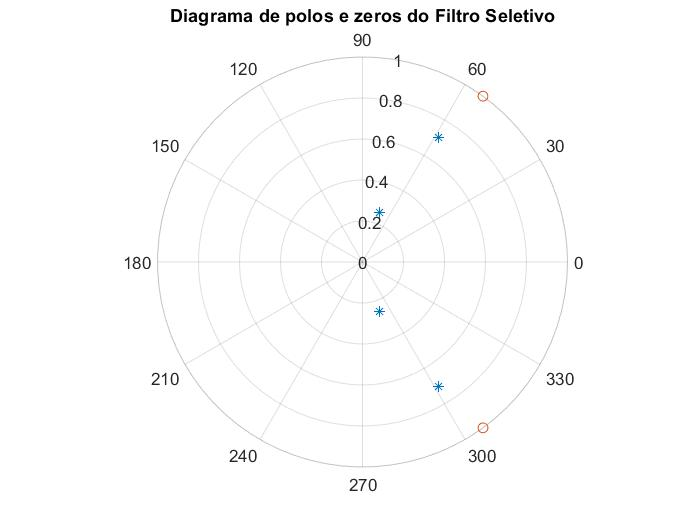
\includegraphics[width=13.5cm]{ex1-pz}
\caption{Diagramas de polos e zeros do filtro seletivo.}
\label{ex1:polos}
\end{figure}
\vspace{0.4cm}

A partir dos polos e zeros é possível plotar a curva da resposta em frequência, como na Figura \ref{ex1:H}. Dela vê-se que tem-se o propósito de atenuar a frequência digital de $\dfrac{3 \pi}{10}$.
\vspace{0.4cm}

\begin{figure}[H]
\centering
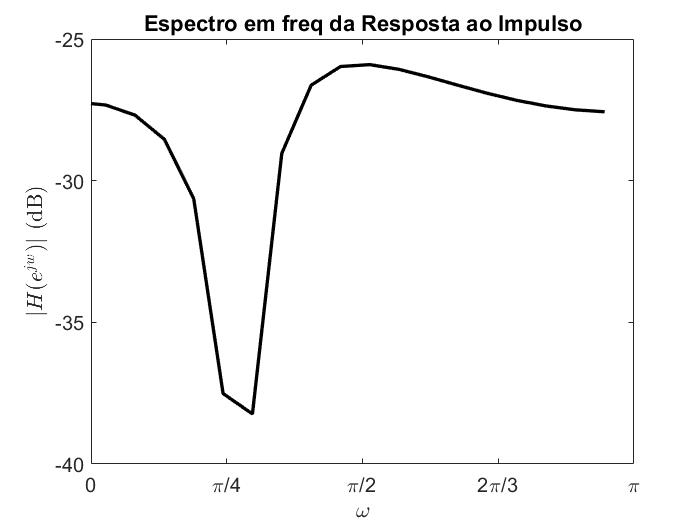
\includegraphics[width=14cm]{ex1-h}
\caption{Resposta em frequência do filtro seletivo.}
\label{ex1:H}
\end{figure}
\vspace{0.1cm}

\subsection{Equação de diferenças e taxa de aquisição}
Considerando uma taxa e aquisição de $F_S=20kHz$ de acordo com o Teorema de Nyquist, pois deve-se ter pelo menos $F_S<2*f_{max}$ para reduzir a distorção significante provocada pelo aliasing. Além disso, a partir dos polos e zeros projetados para eliminar certa frequência, é possível escrever a equação de diferenças correspondente. \\
Com b:
$$0\quad   0\quad   0.0364\quad -0.0427\quad 0.0364$$
e a:
$$1\quad -0.9051\quad 0.6927\quad -0.1318\quad 0.0332$$

\vspace{0.3cm}
\subsection{Comparação entre sinal de entrada e saída}
Aplicando-se a equação de diferenças, ilustrada na Figura \ref{ex1:H}, ao sinal de entrada $x(t)$, tem-se no domínio da frequência a comparação mostrada na Figura \ref{ex1:comp:H} e, após a aplicar a transformar a Transformada Inversa de Fourier para converter novamente para o domínio do tempo, tem-se a comparação vista na Figura \ref{ex1:comp:t}.


\begin{figure}[H]
\centering
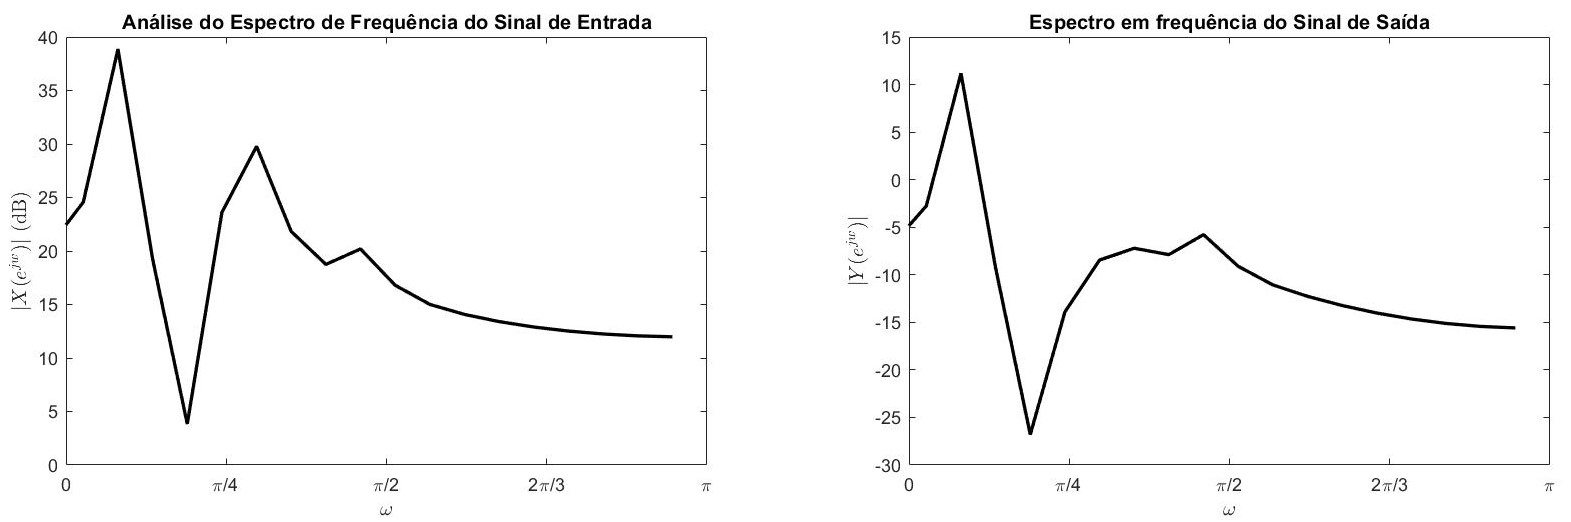
\includegraphics[width=15.5cm]{ex1-comp-H}
\caption{Compração entrada vs. saída no domínio da frequência.}
\label{ex1:comp:H}
\end{figure}
\vspace{0.1cm}

\begin{figure}[H]
\centering
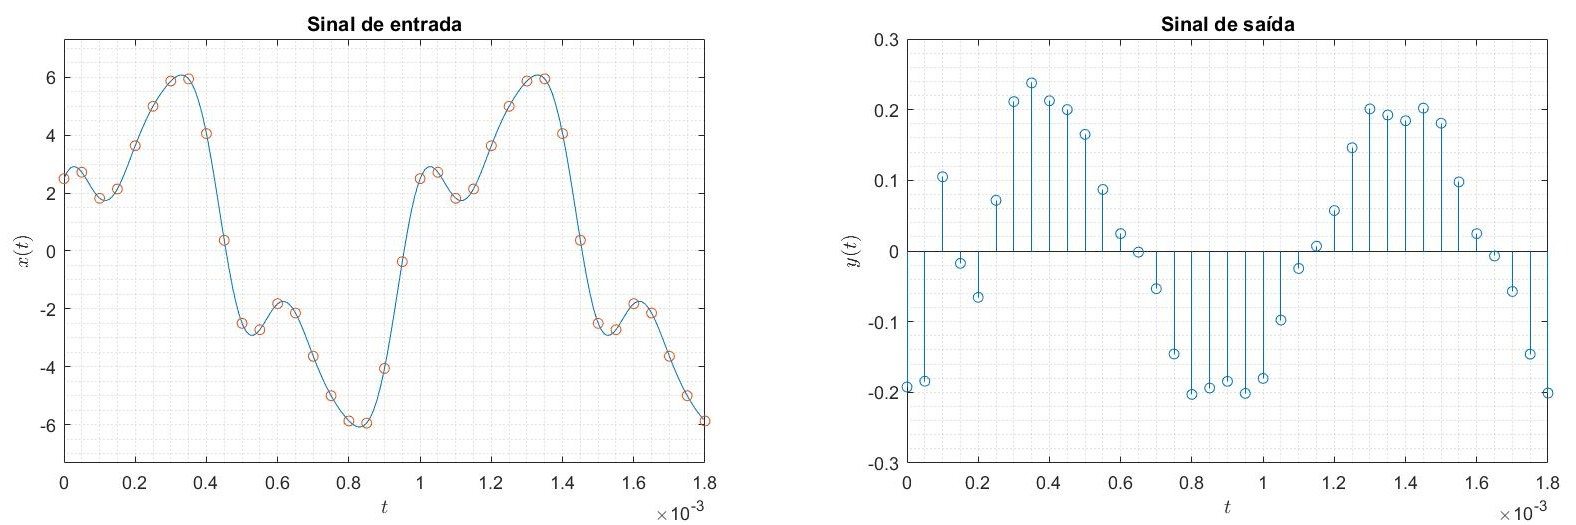
\includegraphics[width=15.5cm]{ex1-comp-t}
\caption{Compração entrada vs. saída no domínio do tempo.}
\label{ex1:comp:t}
\end{figure}
\vspace{0.1cm}

\subsection{Obtenção de saída y(t) por laço for}
A partir dos polos e zeros e zeros determinados tem-se a função de transferência, descrita pela Equação (\ref{ex1:H:pz}). Escolheu-se mais polos que zeros para garantir a estabilidade do sistema.

\begin{equation} \label{ex1:H:pz}
H(z) = 0.0364\  \dfrac{ (z - (0.5877 \pm 0.8089i) )}{(z - (0.0823 \pm 0.2427i))\ (z - (0.3703 \pm 0.6067i))}
\end{equation}
\vspace{0.1cm}

Simplificando \ref{ex1:H:pz} tem-se \ref{ex1:H:ab}, no qual visualizam-se os coeficientes $b$ e $a$.
\vspace{0.1cm}

\begin{equation} \label{ex1:H:ab}
H(z) = \dfrac{Y(z)}{X(z)}=\dfrac{0 - 0\ z^{-1} + 0.0364\ z^{-2} -0.0427\ z^{-3} + 0.0364\ z^{-4}}{1 -0.9051\ z^{-1} +0.6927\ z^{-2} -0.1318\ z^{-3} +0.0332\ z^{-4}}
\end{equation}
\vspace{0.2cm}

Assim, aplicando a transformada de Z inversa, tem-se a equação de diferenças em (\ref{ex1:eqdif}), da qual é possível determinar a saída, como realizado no código em anexo (Anexo \ref{anexo:ex1}) por meio do comando \textbf{\emph{for}}. Ademais, na Figura \ref{ex1:yn} observa-se o resultado obtido, sendo que para as extremidades as distorções levam $y[n]$ a 0 devido a consideração de que para $n<0$, $y[n]=0$.

\begin{multline} \label{ex1:eqdif}
y[n] = 0.9051\ y[n-1] - 0.6927 \ y[n-2]  +0.1318\ y[n-3]  - 0.0332\ y[n-4] \\
+ 0.0364\ x[n-2]   -0.0427\ x[n-3]  +  0.0364\ x[n-4]
\end{multline}

\vspace{0.2cm}
\begin{figure}[H]
\centering
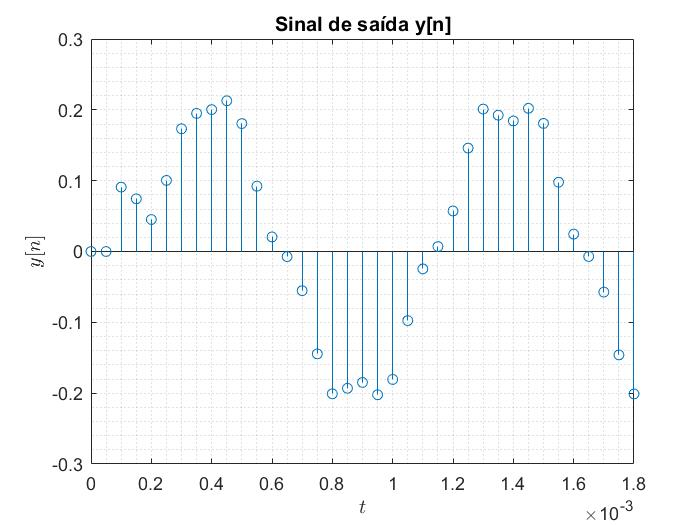
\includegraphics[width=14cm]{ex1_yn}
\caption{Sinal y[n] obtida pela equação de diferenças.}
\label{ex1:yn}
\end{figure}


\vspace{0.5cm}
\section{Exercício 2}
Dada a equação de diferenças tem-se, na Equação (\ref{ex2:eqdif}), sua forma após aplicar-se a Transformada Z. Para assim obter a equação de sua resposta em frequência como na Equação (\ref{ex2:Hz}) e analisá-la no espectro da frequência como na Figura \ref{ex2:H}.

\begin{gather} 
y[n] - y[n-1] + \dfrac{1}{4} y[n-2] = x[n] +\dfrac{1}{4} x[n-1] -\dfrac{1}{8} x[n-2] \label{ex2:eqdif} 
\end{gather}
\begin{gather} 
Y(z)\ (1 - 1\ z^{-1} + 0.25\ z^{-2}) = X(z)\ (1 + 0.25\ z^{-1} + 0.125\ z^{-2})
\end{gather}

\begin{equation} \label{ex2:Hz}
H(z) = \dfrac{1 + 0.25\ z^{-1} + 0.125\ z^{-2}}{1 - 1\ z^{-1} + 0.25\ z^{-2}}
\end{equation}

\vspace{0.4cm}
\begin{figure}[H]
\centering
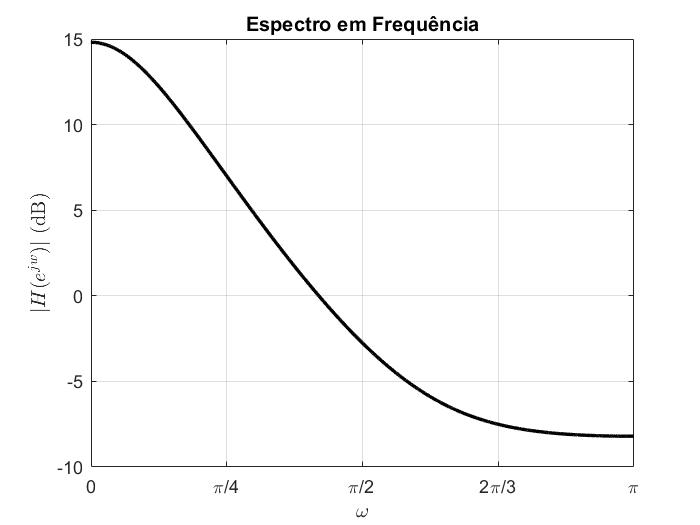
\includegraphics[width=14cm]{ex2-Hz}
\caption{Espectro em frequência da equação de diferenças.}
\label{ex2:H}
\end{figure}

\vspace{0.4cm}
\subsection{Estabilidade do sistema}
A resposta em frequênia do sistema tabém pode ser escrita como mostrado na Equação (\ref{ex2:pz}), na qual observa-se a posição dos polos e zeros. Como há mais polos que zeros a primeira condição para a estabilidade foi obedecida, além de que os polos estão contidos no círculo de raio unitário. Também verifica-se da Figura  \ref{ex2:H} a estabilidade do sistema, uma vez que entradas limitadas gerarão saídas limitas, que conforme com o critério de estabilidade BIBO.

\begin{equation} \label{ex2:pz}
H(z) = \dfrac{(z-(-0.1250 \pm 0.3307i))}{(z-0.5)\ (z-0.5)}
\end{equation}
 
\vspace{0.5cm}
\subsection{Resposta ao degrau}
A resposta degrau foi obtida pela equação de diferenças, a partir da Tranformada Z inversa de \ref{ex2:Hz} e observa-se na Figura \ref{ex2:u}.

\vspace{0.3cm}
\begin{figure}[H]
\centering
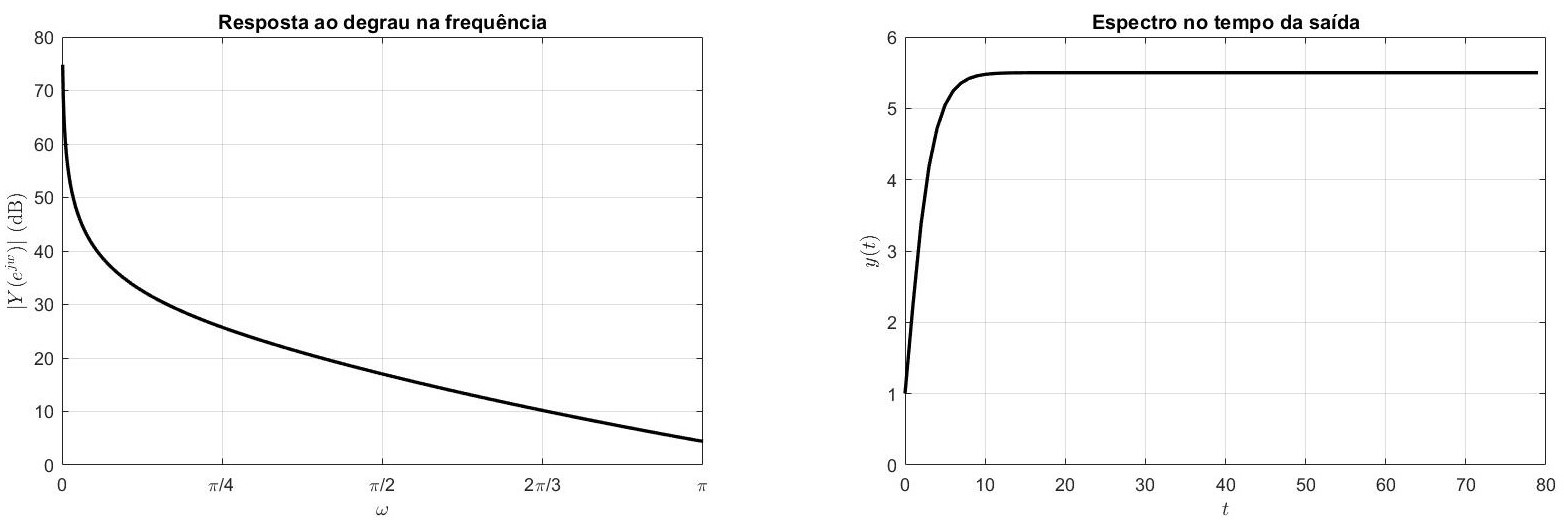
\includegraphics[width=15.8cm]{ex2-u}
\caption{Espectro em frequência e tempo da resposta ao degrau unitário.}
\label{ex2:u}
\end{figure}

\vspace{0.5cm}
\section{Exercício 3}
\subsection{Análise da função de transferência do motor}
Para a análise do sistema do motor em que a entrada é a tensão e a saída, a velocidade angular, tem-se os gráficos das Figuras \ref{ex3:Hjw}, \ref{ex3:ht} e \ref{ex3:st}. Percebe do gráfico da função de transeferência que primeiramente ocorre o acionamento do motor por uma elevada tensão positiva, para depois estabilizar-se e tende a valores proxóimos ao zero. Ademias, do gráfico da resposta ao degrau na Figura \ref{ex3:st}, tem-se que o sistema é subamortecido.

\vspace{0.2cm}
\begin{figure}[H]
\centering
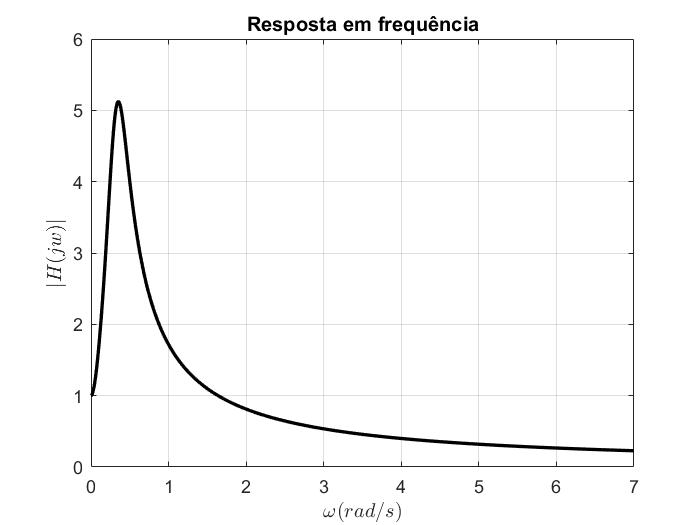
\includegraphics[width=14cm]{ex3-Hjw}
\caption{Espectro em frequência da função de tranferência.}
\label{ex3:Hjw}
\end{figure}

\vspace{0.2cm}
\begin{figure}[H]
\centering
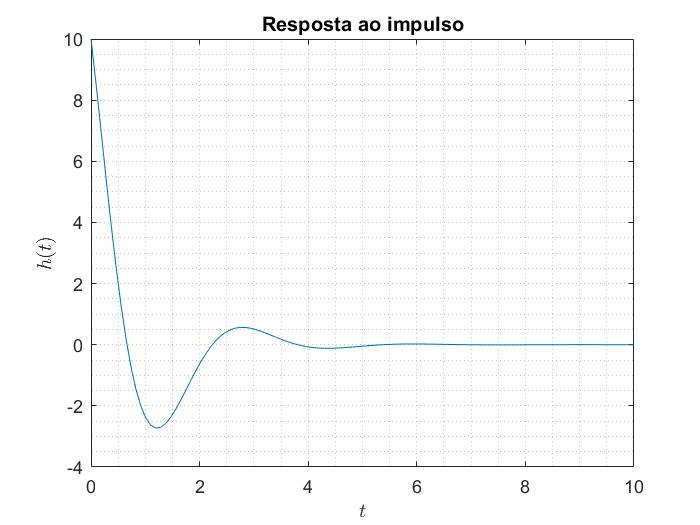
\includegraphics[width=14cm]{ex3-ht}
\caption{Curva de resposta ao impulso.}
\label{ex3:ht}
\end{figure}

\vspace{0.2cm}
\begin{figure}[H]
\centering
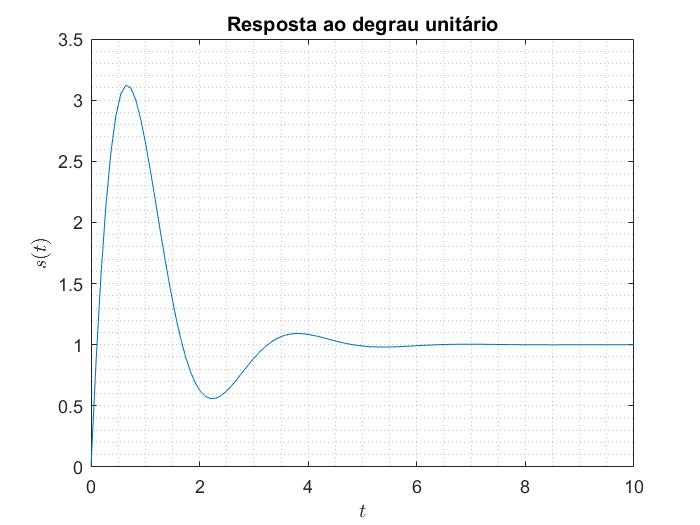
\includegraphics[width=14cm]{ex3-st}
\caption{Curva de resposta ao degrau.}
\label{ex3:st}
\end{figure}

\vspace{0.3cm}
\subsection{Redução de \emph{overshoot}}
Da equação de transferência fornecida para o motor, é possível modelá-la de forma que fique no formato de:

$$H(jw) =\dfrac{\omega_n ^2}{(jw)^2 + 2 \zeta \omega_n (jw)+ w_n ^2} $$

\vspace{0.3cm}
sendo o valor percentual do overshoot dado por: 

$$ M_p = e^{\dfrac{-\zeta\ \pi}{\sqrt{(1-\zeta^2)}}}$$

ou ainda,

$$ \zeta = \sqrt{\dfrac{ln(M_p)^2}{\pi^2 + ln(M_p)^2}}$$

\vspace{0.45cm}
Assim, para um sistema com $M_p< 0,2$, pois no gráfico de resposta ao degrau a estabilização ocorre para s(t)=1, deve-se ter um $\zeta > 0.4559$. Colocando, por exemplo um sistema em série com função de transferência:


$$H_{serie}(j\omega) = \dfrac{5}{(j\omega)+5}$$

\vspace{0.8cm}
Tem-se que os parâmetros para atender a $M_p< 1,2$ estarão na faixa de valores aceitáveis, pois assim ter-se-á $2\zeta\ \omega_n=2 \Rightarrow 2\zeta\ \sqrt{5}=2 \Rightarrow \zeta = 0,4472 \approx 0.4559$. Para esse novo sistema se terá a análise das Figuras \ref{ex3:Hjw:F}, \ref{ex3:ht:F} e \ref{ex3:st:F}, sendo $H_{novo}(jw)$ descrito como na Equação (\ref{ex3:Hnovo}).

\vspace{0.3cm}
\begin{equation} \label{ex3:Hnovo}
H_{novo}(j\omega) = \dfrac{5}{(jw)^2 + 2 \zeta \omega_n (jw) + w_n ^2}
\end{equation}

\vspace{2cm}
\begin{figure}[H]
\centering
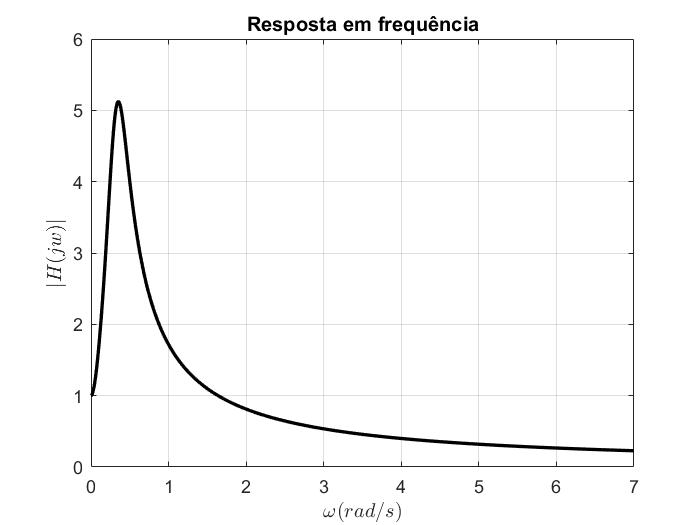
\includegraphics[width=14cm]{ex3-Hjwf}
\caption{Espectro em frequência da função de tranferência para o novo sistema.}
\label{ex3:Hjw:F}
\end{figure}

\vspace{0.2cm}
\begin{figure}[H]
\centering
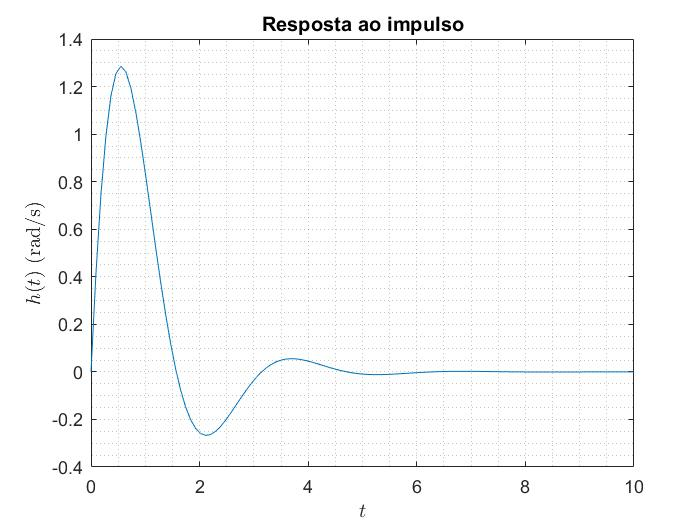
\includegraphics[width=14cm]{ex3-htf}
\caption{Curva de resposta ao impulso para o novo sistema.}
\label{ex3:ht:F}
\end{figure}

\vspace{0.2cm}
\begin{figure}[H]
\centering
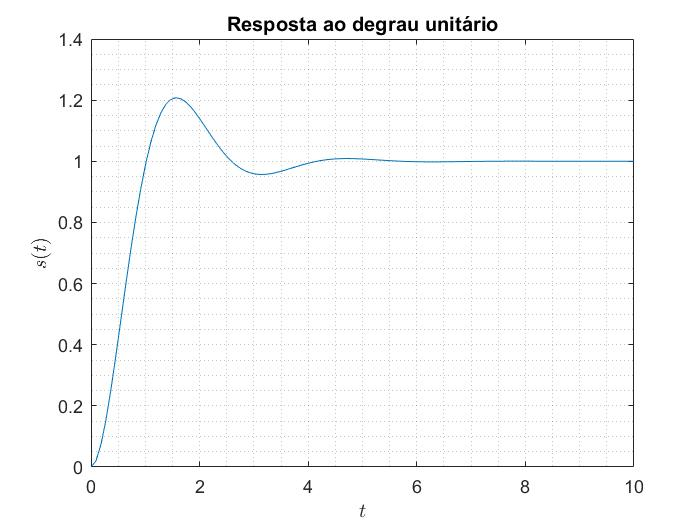
\includegraphics[width=14cm]{ex3-stf}
\caption{Curva de resposta ao degrau para o novo sistema.}
\label{ex3:st:F}
\end{figure}


\vspace{0.3cm}
\subsection{Aumento da velocidade do motor}
Para o aumento da velocidade do motor em 2 vezes, pode-se multiplicar a nova função por dois obtendo-se assim que $2\times H(jw)$ será uma função de transferência com o dobro de ganho, para um inscremento constante de tensão, fazendo assim que a relação entre aumento de tensão e velocidade ângular seja linear. Nas Figuras \ref{ex3:Hjw:F}, \ref{ex3:ht:F} e \ref{ex3:st:F} verifica-se o resultado visual e na Equação (\ref{ex3:Hnovo:2}) a função de tranferência resultante, mantendo $M_p \approx 1,2$.

\vspace{0.4cm}
\begin{equation} \label{ex3:Hnovo:2}
H_{novo}(j\omega) = \dfrac{10}{(jw)^2 + 2 \zeta \omega_n (jw) + w_n ^2}
\end{equation}

\vspace{2cm}
\begin{figure}[H]
\centering
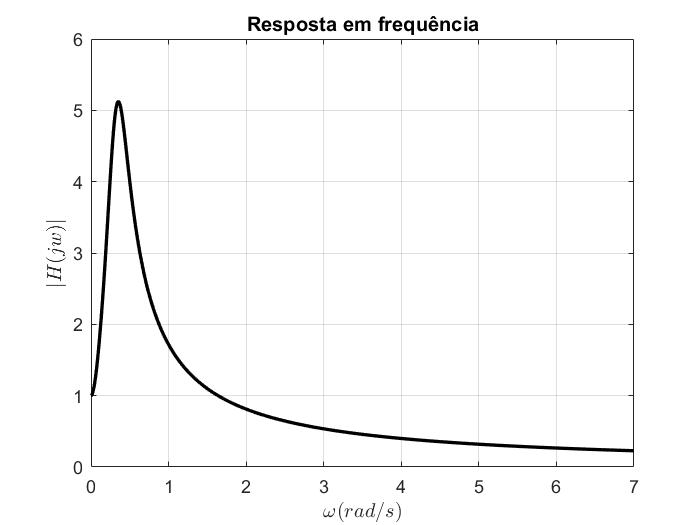
\includegraphics[width=14cm]{ex3-Hjw2}
\caption{Espectro em frequência da função de tranferência para o novo sistema com ganho 2.}
\label{ex3:Hjw:F}
\end{figure}

\vspace{0.2cm}
\begin{figure}[H]
\centering
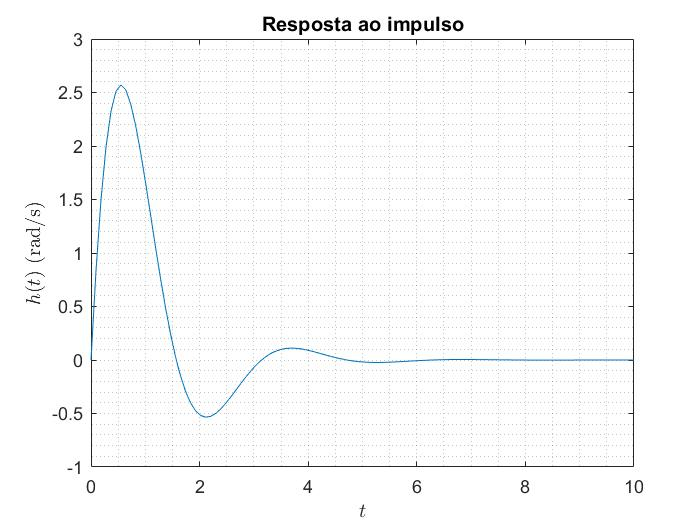
\includegraphics[width=14cm]{ex3-ht2}
\caption{Curva de resposta ao impulso para o novo sistema com ganho 2.}
\label{ex3:ht:F}
\end{figure}

\vspace{0.2cm}
\begin{figure}[H]
\centering
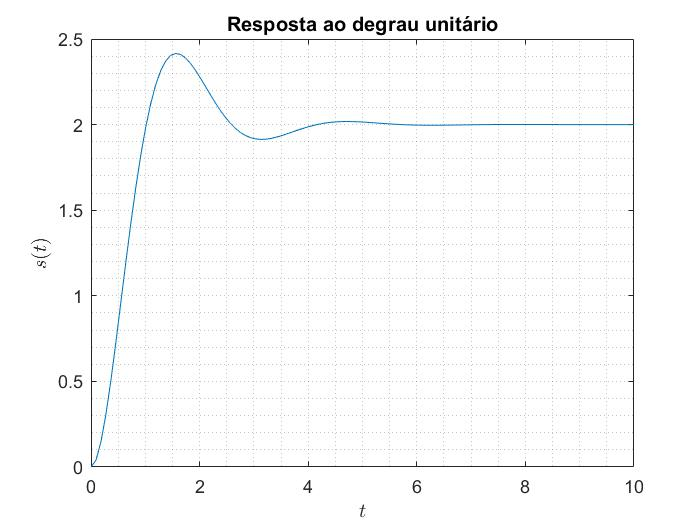
\includegraphics[width=14cm]{ex3-st2}
\caption{Curva de resposta ao degrau para o novo sistema com ganho 2.}
\label{ex3:st:F}
\end{figure}


\section{Exercício 4}
Para um $M_p < 0.25$, tem-se que $\zeta > 0.4037$ idealmente. Ademais, é pedido que $K$ e $a$ sejam projetados de forma que o tempo de acomodação $t_s$ seja igual ou inferior a 0.1s, logo, ainda tem-se que:

$$t_s=\dfrac{4,6}{\zeta \omega_n} \Rightarrow \omega_n=\dfrac{4,6}{\zeta t_s} \Rightarrow \omega_n = 113,9424$$
\vspace{0.3cm}

Para cumprir com esses requisitos idealmente teria-se:

\vspace{0.1cm}
\begin{equation} 
H_{ideal}(j\omega) = \dfrac{144^2}{(jw)^2 + 2 * 0.4037 *144 (jw) + (114) ^2}
\end{equation}
\vspace{0.3cm}

que comparando com a função de transferência de descrita por:

\vspace{0.2cm}
\begin{equation} 
H_{real}(j\omega) = \dfrac{100\ K}{(jw)^2 + (a+25)\ (jw) + 25a}
\end{equation}

\vspace{0.1cm}
tem-se:

\begin{equation*}
\begin{cases}
a+25=2\ \zeta \ \omega _{n}\\
\sqrt{25\ a} =\omega _{n} =\sqrt{100\ K}
\end{cases}
\end{equation*}
\vspace{0.4cm}

das se quais de tira que $a=519.3148$ e $k=129.8287$. Além disso, do código no Anexo \ref{anexo:ex4}, não há zeros e tem-se polos reais em -519.3148 e
  -25.0000, os quais são representados na Figura \ref{ex4:zp}. 

Na Figura \ref{ex4:st}, tem-se ainda a resposta ao degrau unitário da função de transferência resultante e descrita na Equação (\ref{ex4:Hideal})

\vspace{0.4cm}
\begin{equation} \label{ex4:Hideal}
H_{real}(j\omega) =\dfrac{1298,3}{(jw)^2 + (544.3)\ (jw) + 1298,3}
\end{equation}

\vspace{0.4cm}
\begin{figure}[H]
\centering
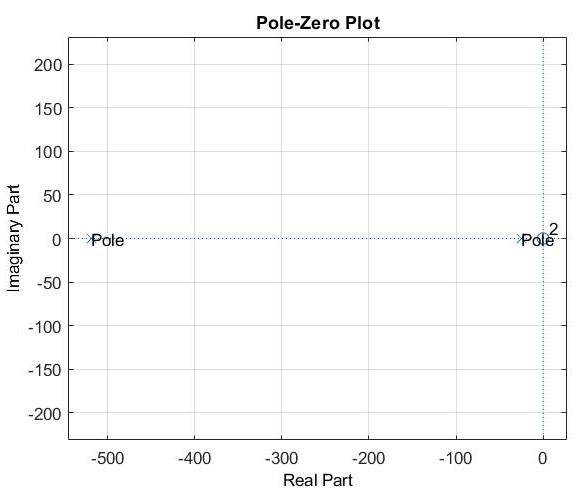
\includegraphics[width=13.5cm]{ex4-zp}
\caption{Curva de resposta ao degrau unitário.}
\label{ex4:zp}
\end{figure}

\vspace{0.2cm}
\begin{figure}[H]
\centering
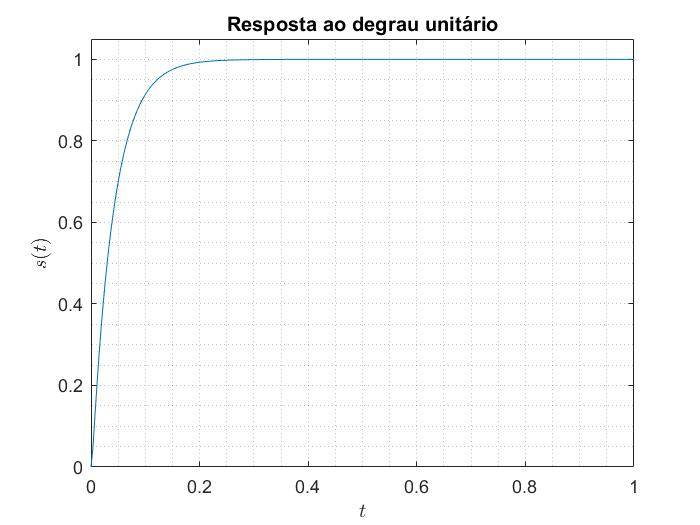
\includegraphics[width=14cm]{ex4-st}
\caption{Curva de resposta ao degrau unitário.}
\label{ex4:st}
\end{figure}

\section{Exercício 5}
Os dados do sistema do laboratório são lineares, no entanto ainda é possível ajustá-ia uma curva, mediante a modelagem exponencial (Veja Anexo \ref{anexo:ex5}). Assim, tem-se que $y(t)$ pode ser descrita como:

$$y(t) = 0.9729\  e^{0.0050\ t} +   0.4321\  e^{-4.0703\ t}      -1.4031\  e^{-1.0747\ t}   $$

Além disso, a Figura \ref{ex5:fig1} mostra a correspondência da curva obtida e a dispersão dos dados, enquanto que na Figura \ref{ex5:fig2} está comtemplado o Diagrama de Bode para o sistema.
\vspace{0.2cm}

\begin{figure}[H]
\centering
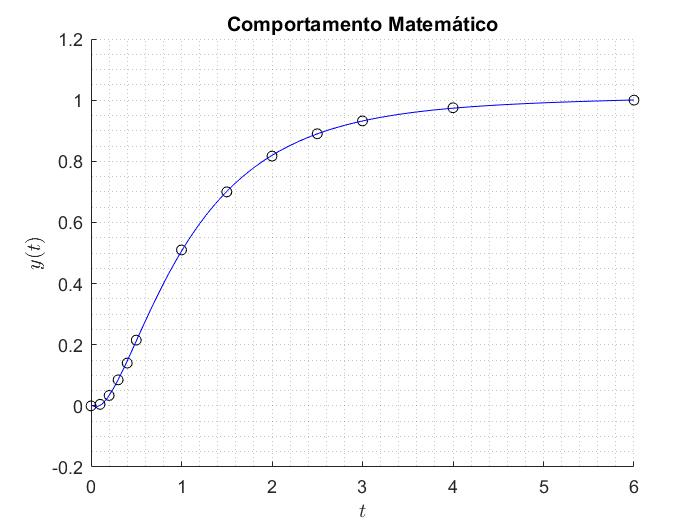
\includegraphics[width=14cm]{ex5-comp-mat}
\caption{Modelagem matemática do sistema via MATLAB.}
\label{ex5:fig1}
\end{figure}

\begin{figure}[H]
\centering
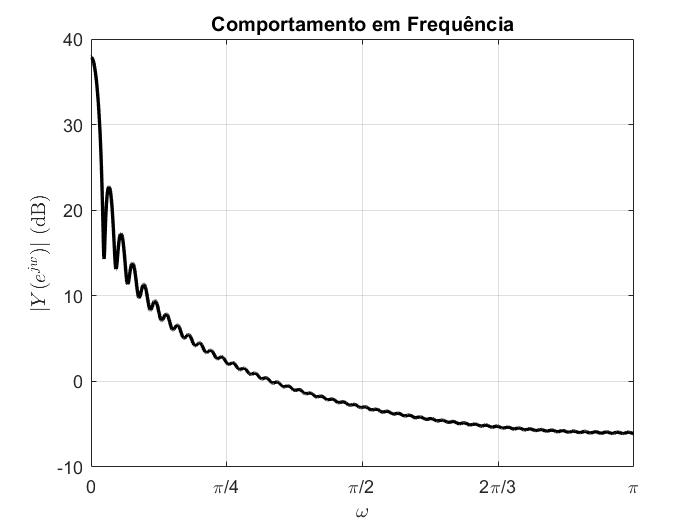
\includegraphics[width=14cm]{ex5-comp-f}
\caption{Comportamento em frequência do sistema.}
\label{ex5:fig2}
\end{figure}

\newpage
\section{Anexos}
\subsection{Código correspondente ao exercício 1} \label{anexo:ex1}
\lstinputlisting{EX1/EX1.m}

\vspace{0.3cm}
\subsection{Código correspondente ao exercício 2} \label{anexo:ex2}
\lstinputlisting{EX2/EX2.m}

\vspace{0.3cm}
\subsection{Código correspondente ao exercício 3} \label{anexo:ex3}
\lstinputlisting{EX3/EX3.m}

\vspace{0.3cm}
\subsection{Código correspondente ao exercício 4} \label{anexo:ex4}
\lstinputlisting{EX4/EX4.m}

\vspace{0.3cm}
\subsection{Código correspondente ao exercício 5} \label{anexo:ex5}
\lstinputlisting{EX5/EX5.m}

\newpage
\begin{thebibliography}{9} 
% Introdução
\bibitem{S1}
    Gene F. Franklin, J. David Powell, Abbas Emami-Naieni.,
    “Sistemas de Controle para a Engenharia”, Porto Alegre: Bookman, 2013.

\bibitem{S2}
    Oppeinheim, Alan V.; Willsky, Allan S.,
    “Sinais e Sistemas”, São Paulo: Pearson
Prentice Hall, 2010. 2ª Edição.

\end{thebibliography}
\end{document}
